\documentclass[a4paper,12pt]{article}
\usepackage{amssymb}
\usepackage{geometry}
\usepackage{graphicx}
\usepackage{colortbl}
\usepackage{wrapfig}
\geometry{margin=1in}



\begin{document}

Dustin Kane

CMSI 370-01

November 24, 2015

\begin{center}
\section*{Assignment 1124: Dream Design}
\subsection*{The Ultimate Heads-Up Display with Microsoft HoloLens}
\end{center}

\section{A Bicycle For Our Minds}

Steve Jobs, the cofounder of Apple Computers, liked to tell a story. He found a study that measured the distance versus energy consumption for various animals. The study found the condor to be the most efficient animal and put humans fairly far down the list. However, Scientific American decided to test the efficiency of a human on a bicycle. A person on a bicycle was by \emph{far} the most efficient animal on the planet. With that in mind, Steve Jobs said this:

\begin{quote} 
    ``And that's what a computer is to me. What a computer is to me is it's the most remarkable tool that we've ever come up with, and it's the equivalent of a bicycle for our minds.'' - Steve Jobs [1]
\end{quote}

Computers are bicycles for our minds. They are augmentations to our intellect. Or, at least they should be. Computers today do not really achieve this vision. The Scientific American test implied that the bicycle was the extension of a person; a person \emph{on} a bicycle \emph{is} the most efficient animal. A modern computer is not an extension of a person. It is a tool: an interface that a person has to interact with. A computer is more like a parking meter or a cashier at a store; it isn't an extension of the person using it by any stretch of the imagination. Smart phones feel more like an extension of a person; people are tethered to their phones and sometimes filter every thought and action through it. But the way they interface with it is still like the way they interact with a garage-door opener or a television remote. Computers are incredibly useful, but their interfaces are essentially just consoles: a set of buttons and switches that make the machine do something. To create an interface that lives up to the dream of the Bicycle of the Mind, we need an interface that we feel connected to and integrated with.

To put it in more concrete terms, a bicycle takes the existing human behavior of movement and improves it by making it faster and more efficient. A computer should take existing human mental behavior and improve it by making it faster, more efficient, and even more. Instead of giving you turn-by-turn directions through Google Maps, the computer should improve your ability to \emph{know} where to go. Instead of allowing a user to look up an actress on IMBD, a computer should improve the ability of the user to \emph{remember} what movies she was in. Instead of providing the user with a calculator, the computer should improve the ability of the user to \emph{calculate} arithmetic problems. I'm not suggesting the computer augment the brain to be more effective; that would be like suggesting a bicycle allows a man to move his legs faster. The problem is the way we interact with computers is more akin to the way we interact with a servant or a secretary: we ask it questions and we give it commands. We do not interact with a bicycle by telling it to go faster: we interact with a bicycle by moving our legs in a way that is fairly similar to the way we would move them without the bicycle, and the bicycle augments that behavior. In the same way, we should interact with a computer by, essentially, doing what we do without a computer and the computer handles the rest.

I imagine a computer that, instead of a screen, superimposes information on our field of vision through a pair of glasses. The computer sees what we see and hears what we hear. We give the computer instructions by, essentially, thinking out loud. Just like we slightly alter the motion of running to apply it to a bicycle, we slightly alter our way of thinking to apply it to this interface. I believe this kind of interface could be created today using the existing concept of a ``Heads-Up Display'' [2] and implementing it with the Microsoft HoloLens hardware [3].

\section{The Heads-Up Display}

\begin{wrapfigure}{r}{0.5\textwidth}
\centering
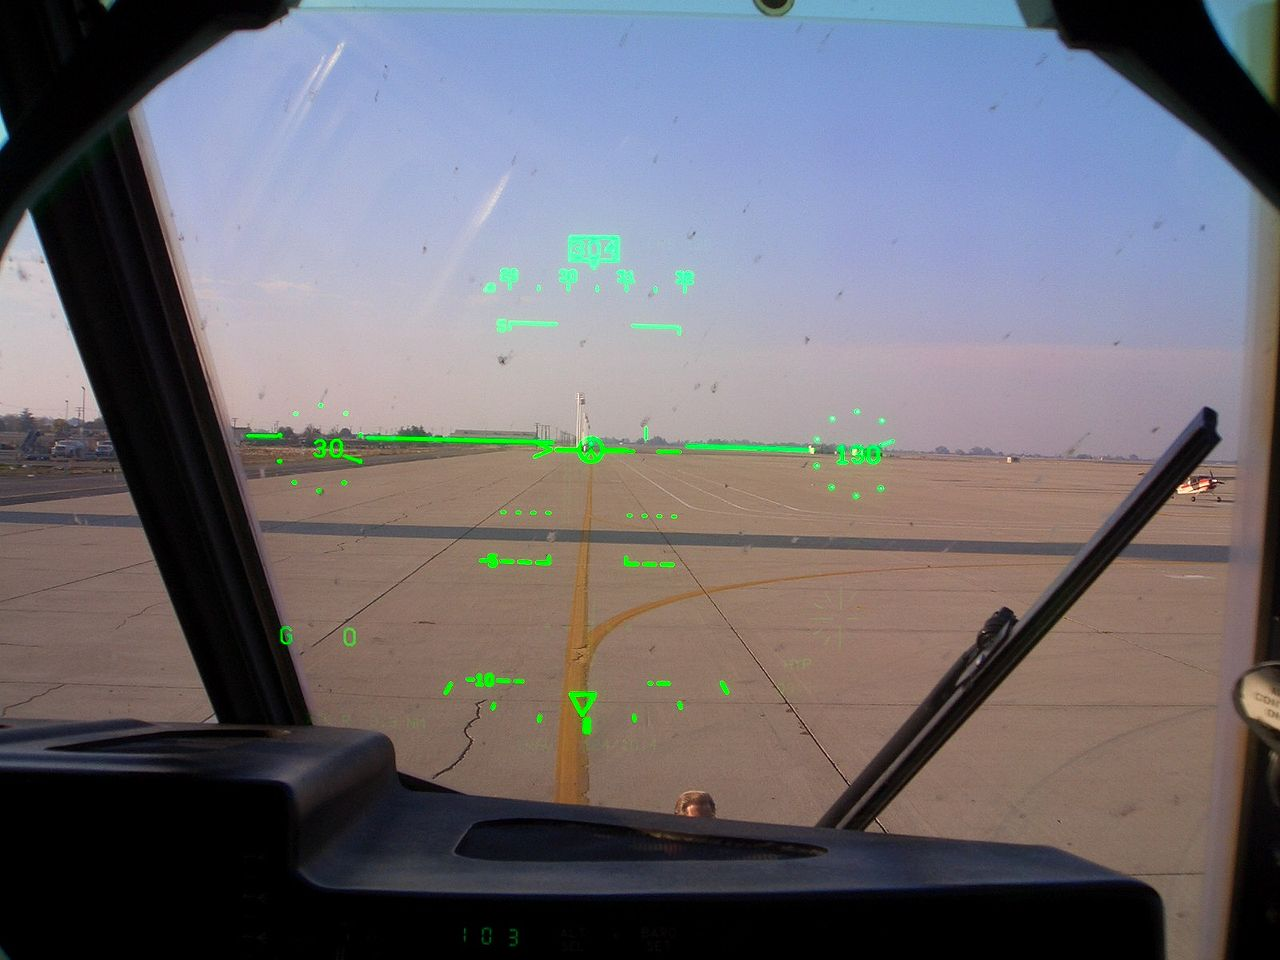
\includegraphics[width=0.5\textwidth]{jethud}
\caption{HUD of a C-130J (https://en.wikipedia.org/wiki/Head-up\_display\#/media/File:C-130J\_Co\_Pilot\%27s\_Head-up\_display.jpg)}
\end{wrapfigure}

A Heads-Up Display is a kind of instrument that super-imposes information over what the user would otherwise be looking at. This kind of instrument is mostly used in military aircraft. The fighter jet has a transparent screen in the cockpit between the pilot and the front windshield. The pilot can now look at readings from his instruments while looking straight ahead; he doesn't have to look down at his instruments, he keeps his head up, hence the name Heads-Up Display.

This interface does more than save the pilot from having to move his head. Like the bicycle, the jet is meant to be an extension of the human being. The pilot looks straight forward at where he's flying. With the Heads-Up display, instead of interacting with his instruments in a kind of transactional way--looking down at them, querying them for information--the pilot has the relevant information right in front of him. The action of the pilot is the same as if the instruments weren't there, yet he still gets the benefit of having the information from them. This kind of interface achieves the dream: 

\section{Sources}

``The holograms you’ll see with Microsoft HoloLens can appear life-like, and can move, be shaped, and change according to interaction with you or the physical environment in which they are visible. Use gestures to create, shape, and size holograms. Use your gaze to navigate and explore. Use your voice to communicate with your apps. Microsoft HoloLens understands your movements, gaze, and voice, enabling you to interact with content and information naturally. Using holograms, you can place your digital content, such as apps, information, and even multi-dimensional videos, in the physical space around you, so you can interact with it.''

``The HPU is custom silicon that processes a large amount of data per second from the sensors. Microsoft HoloLens understands gestures and where you look, and maps the world around you, all in real time.''
\begin{enumerate}
    \item https://www.brainpickings.org/2011/12/21/steve-jobs-bicycle-for-the-mind-1990/
    \item https://en.wikipedia.org/wiki/Head-up\_display
	\item https://www.microsoft.com/microsoft-hololens/en-us/faq
	\item https://www.microsoft.com/microsoft-hololens/en-us/hardware
\end{enumerate}


\end{document}